\chapter{Integrali Doppi e tripli}
\section{Domini normali (semplici)}
\begin{defi}
	I domini delle funzioni a più variabili possono presentare una forma di
	regolarità per cui è possibile delimitare la regione da intervalli e grafici
	di funzione. Si parla quindi di dominio semplice o normale rispetto alla
	variabile delimitabile da un intervallo. La normalità di un dominio è molto
	importante in molte definizioni di integrale multiplo e della sua
	risoluzione tramite le formule di riduzione. Inoltre la presenza di un
	dominio regolare permette ulteriori teoremi e formule d'integrazione, come
	le formule di Gauss-Green, il teorema della divergenza e il teorema del
	rotore.
\end{defi}
\subsection{Dominio normale rispetto all'asse $x$}
Il dominio A si definisce {\color{red} normale} rispetto all'asse $x$ se è così
definito:
\begin{equation}
	A=\begin{cases}
		a\leq x\leq b & x \text{ valria in un intervallo}\\
		g_1(x)\leq y\leq g_2(x) & y \text{ varia tra due funzioni di }x
	\end{cases}
\end{equation}
\begin{esempio}
\begin{equation*}
	D=\begin{cases}
		0\leq x\leq 1\\
		x^2\leq y\leq x
	\end{cases}
\end{equation*}
\end{esempio}
Il dominio $B$ si definisce {\color{red} normale} rispetto all'asse $x$ se è così
definito:
\begin{equation}
	A=\begin{cases}
		c\leq y\leq d & y \text{ valria in un intervallo}\\
		h_1(y)\leq x\leq h_2(y) & x \text{ varia tra due funzioni di }y
	\end{cases}
\end{equation}
\begin{esempio}
\begin{equation*}
	D=\begin{cases}
		0\leq y\leq 1\\
		y< x< \sqrt{y}
	\end{cases}
\end{equation*}
\end{esempio}
\subsection{Domini Polarmente normale}
Il dominio C si definisce polarmente normale se è costantemente definito:
\begin{equation}
	C=\begin{cases}
		\theta_1\leq \theta\leq \theta_2 \\
		\varphi_1(\theta)\leq \varphi(\theta)\leq \varphi_2(\theta)
	\end{cases}
\end{equation}
\begin{esempio}
  \begin{equation}
    (x-1)^2+y^2\leq 1
  \end{equation}
  l'angolo varia tra 0 e $\frac{\pi}{2}$, il segmento $\varphi$ dipende dall'angolo
  \begin{equation*}
    \begin{matrix}
      \theta=0\text{ è } \max \varphi=2 \\
      \theta=\frac{\pi}{2} \text{ è } \min \varphi=0 \\
      \varphi=2\cos \theta
      \begin{cases}
        0\leq \theta \leq \frac{\pi}{2}\\
        0\leq \varphi\leq 2\cos \theta
      \end{cases}
    \end{matrix}
  \end{equation*}
  corona circolare $\varphi=r$ $\varphi=R$
  \begin{equation*}
    \begin{cases}
      0\leq \theta \leq \frac{\pi}{2}\\
      r\leq \varphi\leq R
    \end{cases}
  \end{equation*}
\end{esempio}
\subsection{Definizione di integrale doppio}
\begin{defi}
  Sia f(x,y) una funzione limitata nel rettangolo $R=[a,b]x[c,d]$, coordinata in $[a,b]$ e
  di seconda coordinata in $[c,d]$
  Deconpongo regolarmante gli intervalli $[a,b]$ e $[c,d]$,
  \begin{equation*}
    \begin{matrix}
        \text{decomponendo }[a,b]\text{ si ha} & D_1=\{x_0=a,x_1,x_2,\dots,x_n=b\}\\ 
        \text{decomponendo }[c,d]\text{ si ha} & D_1=\{y_0=a,y_1,y_2,\dots,y_n=d\}
    \end{matrix}
  \end{equation*}
  Il prodotto cartesiano $D=D_1*D_2$ è una semidivisione del rettangolo R
  \begin{figure}[ht]
    \centering
    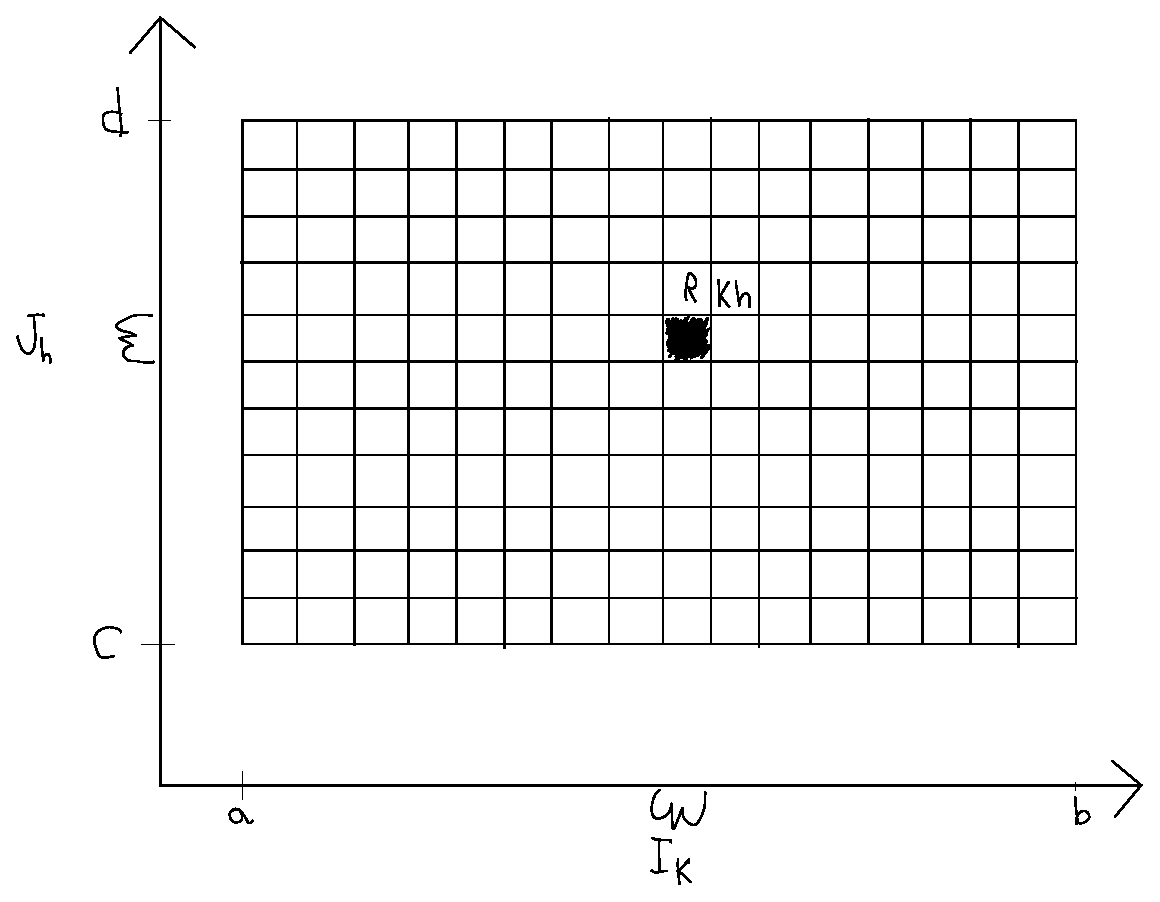
\includegraphics[width=8cm]{img/finiti/graficodecomposizioneR.eps}
    \caption{Decomposizione del rettangolo R}
  \end{figure}
  \begin{equation*}
    \begin{matrix}
        I_k=[x_{k-1},x_k] \text{ in } D_1 (k=1,\dots,n)\\
        J_h=[y_{h-1},y_h] \text{ in } D_2 (h=1,\dots,n)
    \end{matrix}
  \end{equation*}
  Il prodotto cartesiano $I_k*J_h$ individua il generico subrettangolo $R_{kh}$ della semidivisione.\\
  Prendo un generico punto del subrettangolo $R_{kh}(x_k,y_h)$ e faccio il seguente prodotto:
  \begin{equation*}
    f(x_k,y_h)*mis R_{kh} \text{ con } misR_{kh} = misI_k * misJ_h \text{ area del subrettangolo}
  \end{equation*}
  Con l'integrale doppio consudero il volume del parallelepipedo.\\
  Geometricamente considera il pettangolo $R_{kh}$ e la parte di superficie $f(x,y)$ che vi si
  presenta il prodotto $f(x_i,y_n)*mis R_{kh}$ è il volume del parallelepipedo di base $R_{kh}$
  e altezza $f(x_k,y_h)$.
\end{defi}
\section{Somme di Riemann}
Definisco le somme di Riemann $\displaystyle\sum^{k=m\text{ } h=n}_{k=h=1}f(x_k,y_h)*R_{kh}$ ciò
rappresenta la somma di tutti i volumi dei parallelepipedi di base $R_{kh}$ e altezza $f(x_k,y_h)$
che si possono ottenere nel rettangolo $R$.\\
Infittisco le decomposizioni $D_1$ e $D_2(m\to \infty;n\to\infty)$, ottenendo così un numero sempre
maggiore di subrettangoli di ampiezza via via minore.
\begin{equation}
  mis R_{kn}=misI_k*misI_n=\frac{b-a}{m} * \frac{d-c}{n}\to 0 \text{ per }  m,n \to \infty
\end{equation}
Con l'infittirsi della decomposizione, aumenta la precisione con cui ciascun parallelepipedo
approssima il volume sotto al grafico delle funzione in ogni $R_{kh}$.\\
Al limite, le somme di Riemann daranno il volume sotto al grafico della funzione in un certo
rettangolo (in generale dominio).\\
Se esiste finito $\lim\limits_{n\to \infty\text{ } m\to \infty}\displaystyle\sum_{h=k=1}^{k=m\text{ }h=n}f(x_k.y_n)*misR_{kh}$ tale limite è definito \underline{\color{red} ingrale doppio} di f(x,y) nel
dominio $R=[a,b]*[c,d]$
\begin{equation}
  \iint_R f(x,y)dxdy=\lim\limits_{n\to \infty\text{ } m\to \infty}\displaystyle\sum_{h=k=1}^{k=m\text{ }h=n}f(x_k.y_n)*misR_{kh}
\end{equation}
\paragraph{Somme superiori e somme inferiori}
\begin{defi}
  È possibile definire l'integrale doppio anche con le somme superiori e le somme inferiori
  \begin{equation*}
    \text{Somme inferiori } s(f,R) = \displaystyle\sum inf_{R_{kh}}f(x_k.y_n)*misR_{kh}
  \end{equation*}
  prendo il minimo valore che la funzione assume nel subrettangolo $R_{kh}$ e lo moltiplico per
  l'area di tale subrettangolo. Sommando ottengo un parallelepipedo, il cui volume approssima
  per difetto individuato dalla funzione. 
  \begin{equation*}
    \text{Somme superiori } s(f,R) = \displaystyle\sum sup_{R_{kh}}f(x_k.y_n)*misR_{kh}
  \end{equation*}
  prendo il massimo valore che la funzione assume nel subrettangolo $R_{kh}$ e lo moltiplico per
  l'area di tale subrettangolo. Sommando ottengo un parallelepipedo, il cui volume approssima per
  eccesso quello individuato dalla funzione all'infittirsi della decomposizione le somme inferiori
  crescono, le somme superiori decrescono. Le somme superiori e le somme inferiori convergono ad
  uno stesso valore, detto {\color{red}integrale doppio}\footnote{è il valore sotto al grafico
    della funzione}
  \begin{equation*}
    \lim s=\lim S=\iint_R f(x,y)dxdy
  \end{equation*}
\end{defi}
\clearpage
\subsection{Proprietà dell'integrale doppio}
\begin{equation*}
  \begin{matrix}
  \text{Linearità } \begin{cases}
                      1) \iint_D [f_1(x,y)+f_2(x,y)]dxdy=\iint_Df_1(x,y)dx*dy+\iint_Df_2(x,y)dx*dy\\
                      2) \iint_D \alpha f_1(x,y)dxdy=\alpha\iint_Df_2(x,y)dx*dy
                    \end{cases}\\
    \text{Assitività } 3)\text{ Sia } D=D_1\cup D_2 \iint_Df(x,y)dxdy=\iint_{D_1}f(x,y)dx*dy +\iint_{D_2}f(x,y)dx*dy\\
    \text{Monotonia } \begin{cases}
                        4) \text{ Sia } f(x,y)\leq g(x,y)\text{ } \forall (x,y) \in D\\
                        \text{ }\iint_Df(x,y)dxdy \leq \iint_Dg(x,y)dx*dy\\
                        5) \text{ Sia } D_1 \subset D\\
                        \text{ } \iint_{D_1}f(x,y)dxdy < \iint_Df(x,y)dx*dy \\
                        6) \abs{\iint_Df(x,y)dxdy} \leq \iint_D\abs{f(x,y)}dx*dy
                      \end{cases}
  \end{matrix}
\end{equation*} 

\subsection{Formula di riduzione}
\begin{itemize}
\item Sia $A\subset R^2$ un dominio normale rispetto all'asse x
  \begin{equation*}
    A=\begin{cases}
        a\leq x\leq b\\
        g_1(x)\leq y\leq g_2(x)
      \end{cases}
  \end{equation*}
    Allora $\iint_A f(x,y) dxdy=\int_a^bdx \left(\int_{g_1(x)}^{g_2(x)}f(x,y)dy\right)$\\
    calcolo prima $\int_{g_1(x)}^{g_2(x)}f(x,y)dy$ che è una funzione della sola $x$ $\not{o}(x)$
    \begin{equation*}
      \text{per calcolo } \int^b_a \not{o} (x) dx
    \end{equation*}
  \item Dominio polarmente normale\\
    Effettua un cambio di coordinate, passando dalle coordinate cartesiane a quelle polari
    \begin{equation*}
      \text{L'integrale doppio è } \iint_Df(x,y)dxdy
    \end{equation*}
    Passando alle coordinate polari
    \begin{equation*}
      \begin{matrix}
        \text{del dominio } D(x,y) \text{ passerò al dominio } D^\prime (\varphi, \theta) \\
        \text{della funzione } f(x,y) \text{ passerò al dominio } f (\varphi, \theta)
      \end{matrix} \begin{cases}
                       x=\varphi\cos\theta\\
                     y=\varphi\sin\theta
                   \end{cases}
                   \varphi=\sqrt{x^2+y^2} 
   \end{equation*}
   e da differenziali $dxdy$ passerò ai differenziali $d\varphi d\theta$. \\
   Si dimostra che nel passaggio ad altre coordinate il differenziale è $\abs{j} d\varphi d\theta$,
   dove $\abs j$ è il determinante della {\color{red} matrice Jacobiana} che contiene le derivate
   parziale prime
   \begin{equation}
     \abs{J}=\begin{vmatrix}
               x_\varphi & x_\theta\\
               y_\varphi & y_\theta
             \end{vmatrix}
             \to \abs{J}=\begin{vmatrix}
                           \cos \theta & -\varphi \sin \theta\\
                           \sin \theta & \varphi \cos \theta
                         \end{vmatrix}
                         =\varphi\cos^2\theta+\varphi \sin^2\theta =\varphi
   \end{equation} 
   Per cui passando da $dxdy$ alle coordinate polari avrò $\varphi d\varphi d\theta$ così
   l'integrale doppio diventa:
   \begin{equation*}
     \iint_Df(x,y)dxdy=\iint_{D^\prime}f(\varphi,\theta)\varphi d\varphi d\theta
   \end{equation*}
\end{itemize}
\clearpage
\subsubsection{Esempi di domini polarmente normali}
\begin{figure}[ht]
  \centering
  \includegraphics[width=14cm]{img/finiti/esdompolnorm.eps}
  \caption{Esempi di domini polarmente normali}
\end{figure}
\subsection{Baricentro di un dominio normale}
\begin{defi}
  Sia D un demonio normale del piano. Si definisce {\color{red}baricentro del dominio} D il punto di
  coordinate $(x_0,y_0)$ tale che:
  \begin{equation*}
    \begin{matrix}
      x_0=\frac{1}{mis D} \iint_D xdxdy & y_0=\frac{1}{mis D} \iint_D ydxdy
    \end{matrix}
  \end{equation*}
  $mis D:$ misura ({\tt area}) del dominio $D$.
\end{defi}
\begin{esempio}
  calcolare il baricertro del dominio $D=\begin{cases}
                                           0\leq x\leq 2\\
                                           0\leq y\leq 1
                                         \end{cases}$
  \begin{equation*}
    mis D=A_{rettangolo}=2*1=2
  \end{equation*}
  \begin{figure}[ht]
    \centering
    \includegraphics[width=6cm]{img/finiti/baricentrodiundominionormale.eps}
    \caption{Baricentro di un dominio normale}
  \end{figure}
  \begin{equation*}
    \begin{matrix}
      x_0=\frac{1}{mis D}\iint_D xdxdy=\frac{1}{2}\int_0^2dx\int_0^1xdy=\frac{1}{2}\int^2_0dx\abs{xy}_0^1= \frac{1}{2}\int_0^2xdx=\frac{1}{2}\abs{\frac{x^2}{2}}_0^2=\frac{1}{\not{2}}\not{2}=1\\
      y_0=\frac{1}{mis D}\iint_D ydxdy=\frac{1}{2}\int_0^2dx\int_0^1ydy=\frac{1}{2}\int_0^2dx\left|\frac{y^2}{2}\right|^1_0=\frac{1}{2}\int^2_0\frac{1}{2}dx=\frac{1}{4}\left|x\right|=\frac{1}{2}
    \end{matrix}
  \end{equation*}
  \clearpage
   \begin{center}
            \fbox
            {
            \begin{minipage}{0.85\textwidth}
		Calocolare il baricentro del dominio $D=\begin{cases}
                                                          0\leq \theta \leq \frac{\pi}{2}\\
                                                          0\leq y \leq \sqrt{1-x^2}
                                                          \end{cases}$
              \begin{multicols}{2}
                \includegraphics[width=6cm]{img/finiti/baricentrodiundominionormale2.eps}\\
                \begin{equation*}
                  \begin{matrix}
                    D=\begin{cases}
                      0\leq \theta\leq\frac{\pi}{2}\\
                      0\leq \varphi\leq 1
                    \end{cases} & mis D=\frac{\pi}{4}
                  \end{matrix}
                \end{equation*}
              \end{multicols}
              \begin{equation*}
                \begin{matrix}
                  x_0= \frac{1}{mis D}\iint_D xdxdy=\frac{4}{\pi}
                  \int^{\frac{\pi}{2}}_0d\theta\int_0^1
                  \varphi^2\cos \theta d\theta = \frac{4}{\pi} \int_0^{\frac{\pi}{2}}d\theta \left|
                  \frac{\varphi^3}{3}\cos\theta\right|_0^1\\=\frac{4}{\pi}\int_0^{\frac{\pi}{2}}
                  \frac{1}{3} \cos \theta d\theta = \frac{4}{3}\pi \left|\sin
                  \theta\right|^{\frac{\pi}{2}}_0=\frac{4}{3}\pi\\
                  y_0=\frac{1}{mis D}\iint_D xdxdy=\frac{4}{\pi}
                  \int^{\frac{\pi}{2}}_0d\theta\int_0^1
                  \varphi^2\sin \theta d\theta = \frac{4}{\pi} \int_0^{\frac{\pi}{2}}d\theta \left|
                  \frac{\varphi^3}{3}\sin\theta\right|_0^1\\
                  =\frac{4}{\pi}\int_0^{\frac{\pi}{2}}\frac{1}{3}\sin\theta d\theta =\frac{4}{\pi}*
                  \frac{1}{3}\left|-\cos\theta \right|^{\frac{\pi}{2}}_0=\frac{4}{3}\pi
                \end{matrix}
              \end{equation*} 
            \end{minipage}
            }
  \end{center}
\end{esempio}
\subsection{Domini normali in $R^3$}
\begin{defi}
Il dominio $V$ definisce normale rispetto al piano $xy$ se si può così descrivere:
\begin{equation*}
  \begin{matrix}
    \begin{cases}
      (x,y)\in D & \text{normale}\\
      \alpha(x,y) & \leq z\leq \beta (x,y)
    \end{cases}& \begin{matrix}
                   (x,y) \text{ appartengono ad un dominio normale di } R^2\\
                   z \text{ è compresa tra funzioni di } x \text{ e } y 
                 \end{matrix}
  \end{matrix}
\end{equation*}
$\forall (x,y)\in D$ incontro prma la superficie minorante e per la superficie maggiorante.
\end{defi}
\section{Integrali tripli}
\begin{defi}
  Sia $f(x,y,z)$ una funzione limitata in un insieme $V$, considero il parallelepipedo
  \begin{multicols}{2}
    \begin{equation*}
      V=[a,b]*[c,d]*[e,f]
    \end{equation*}
    Decompongo regolarmente $[a,b],[c,d],[e,f]$\\
    rispettivametne in $n,m e k$\\
    intervalli $I_n=[x_0=a,\dots,x_n=b]$,
    \begin{equation*}
      l_m=[y_0=c,\dots,y_m=d],\text{ } l_k=[z_0=e,\dots,z_k=f]
    \end{equation*}
    \includegraphics[width=4cm]{img/finiti/rettangolo.eps}
  \end{multicols}
  Il prodotto cartesiano $I_n*I_n*I_k$ individua il generico subparallelepipedo $V_{n,m,k}$.
\end{defi}
\clearpage
Definisco le somme di Riemann: $\sum f(x,y,z)*misV_{n,m,k}$\footnote{$misV_{n,m,k}$: misura il
  volume del parallelepipedo}\\
All'infittirsi delle decomposizioni le somme di Riemann convergono ad uno stezzo valore, tale
valore è definito {\color{red}integrale triplo} di $f(x,y,z)$ in $V$
\begin{equation*}
  \lim_{m\to \infty\text{ } n \to \infty \text{ } k\to \infty}\sum f(x,y,z) misV_{n,m,k}=\iiint_V f(x,y,z)dxdydz
\end{equation*}
Oppure, definisco le somme inferiore e le somme superiori
\begin{equation*}
  \begin{matrix}
    \text{Somme inferiori} &\sum misV_{n,m,k}*\min_{V_{n,m,k}}f(x,y,z)\\
    \text{Somme superiori} &\sum misV_{n,m,k}*\max_{V_{n,m,k}}f(x,y,z)
  \end{matrix}
\end{equation*}
All'infittirsi della decomposizione le somme inferiori crescono mentre le somme superiori
decrescono. Se convergono ad una stesso valore, tale valore è definito {\color{red}integrale triplo}
di $f(x,y,z)$ in $V$
\begin{equation*}
  \lim s(f,V)= \lim S(f,V)= \iint_V f(x,y,z) dxdydz
\end{equation*}
\subsection{Formule di riduzione per gli integrali tripli}
Sia $g(x,y)$ integrabile in un dominio normale $V$
\begin{equation*}
  \begin{matrix}
    V=\begin{cases}
        \alpha (x,y) \leq z\leq \beta (x,y)\\
        (x,y)\in D
      \end{cases} & \iiint_V f(x,y,z) dxdydz = \iint_D dxdy \displaystyle\int_{a(x,y)}^{\beta (x,y)} f(x,y,z)dz
  \end{matrix}
\end{equation*}
Se il dominio $D$ è normale rispetto all'asse $x$
\begin{equation*}
	V=\begin{cases}
		a\leq x\leq b\\
		g_1(x)\leq y\leq g_2(x)\\
		\alpha (x,y) \leq z \leq \beta (x,y)
	\end{cases} \iiint_V f(x,y,z) dxdydz = \int_\theta^\theta dx
	\int_{f_1(x)}^{f_2(x)}dy\int_{\alpha(x,y)}^{\beta(x,y)}f(x,y,z)dz
\end{equation*}
Se il dominio $D$ è normale rispetto all'asse $y$
\begin{equation*}
	V=\begin{cases}
		c\leq y \leq d\\
		h_1(y)\leq x \leq h_2(y)\\
		\alpha (x,y) \leq z \leq \beta(x,y)
	\end{cases} \iiint_V f(x,y,z) dxdydz = \int_c^d dy
	\int_{h_1(y)}^{h_2(y)}\int_{a(x,y)}^{\beta(x,y)} f(x,y,z) dz
\end{equation*}
Se il dominio $D$ è polarmente normale
\begin{equation*}
	V=\begin{cases}
		\theta_1\leq \theta \leq \theta_2\\
		\varphi_1(\theta)\leq \varphi \leq \varphi_2(\theta)\\
		\alpha (\varphi,\theta)\leq z \leq \beta(\varphi,\theta)
	\end{cases} \iiint_V f(x,y,z)dxdydz=\int_{\theta_1}^{\theta_2}d\theta
	\int^{\varphi_2(\theta)}_{\varphi_1(\theta)} \varphi d \varphi
	\int^{\beta(\varphi, \theta)}_{\alpha (\varphi,\theta)}
	f(\varphi,\theta,z)dz 
\end{equation*}
\begin{equation*}
	\begin{matrix}
		\alpha(x,y)&\to&\alpha (\varphi, \theta)\\
		\beta (x,y)&\to& \beta(\varphi, \theta)\\
		f(x,y,z) &\to & f(\varphi,\theta, z)\\
		dxdydz &\to & pd\theta d\varphi dz
	\end{matrix}
\end{equation*}
\clearpage
\subsection{Significato geometrico degli integrali}
\begin{equation*}
	\begin{matrix}
		\int & \text{area}\\
		\iint & \text{volume}\\
		\iiint & \text{nessun significato geometrico}
	\end{matrix}
\end{equation*}
\subsection{Coordinate polari e coordinate cilindriche}
$(x,y) \to (\varphi,\theta)$
\begin{equation*}
	\begin{matrix}
		\begin{cases}
			x=\varphi \cos \theta\\
			y=\varphi \sin \theta
		\end{cases} & \varphi =\sqrt{x^2+y^2} &det J=\varphi
	\end{matrix}
\end{equation*}
\paragraph{coordinate alindriche}
$(x,y,z)\to (\varphi,\theta,z)$
\begin{equation*}
	\begin{matrix}
		\begin{cases}
			x=\varphi \cos \theta\\
			y=\varphi \sin \theta\\
			z=z
		\end{cases} & \varphi =\sqrt{x^2+y^2+z^2} &det J=\varphi
	\end{matrix}
\end{equation*}
\paragraph{coordinate sferiche}
\begin{equation*}
	\begin{matrix}
		\begin{cases}
			x=\varphi \sin\theta \cos \alpha\\
			y=\varphi \sin \theta \sin \alpha\\
			z=\varphi \cos\theta
		\end{cases} 
	\end{matrix}
\end{equation*}
\subsection{Interazione per fette}
Considera un volume $V$ e lo interseco con un piano $z=k$. Così ottengo una
sezione $S_z$
\begin{equation*}
	z=1-x^2-y^2
\end{equation*}
Al variare di $z$ tra due valori, cioè facendo variare $S_z$ in funzione di $z$
descrivo il volume $V$.
\begin{esempio}
	\begin{equation*}
		\int_{0}^{1} S_zdz
	\end{equation*}
	$S_z$ è un cerchio di raggio $R(z)$ che depende da $z$
	\begin{equation*}
		\begin{matrix}
			z=1-x^2+y^2 & x^2+y^2=1-z\\
			R^2=1-z & R(z)=\sqrt{1-z}
		\end{matrix}
	\end{equation*}
	$S_z=\pi R^2=\pi(1-z)$
	\begin{equation*}
		\iint_T f(x,y,z)dxdydz=\int_0^1\pi(1-z)dz
	\end{equation*}
\end{esempio}
\subsection{Integrali curvilinei}
\subsubsection{Curve in $R^2$ e in $R^3$}
\begin{defi}
	Si definisce {\color{red}curva} una coppia del tipo $(\gamma,\Gamma)$ con
	\begin{equation*}
		\vec{F}(t)=(x(t),y(t),z(t),\dots) \text{ } t\in [a,b]
	\end{equation*}
	si tratta di un'applicazione $R\to R^n$ ad un valore di $t$ associo $n$
	valori\\
	Le curve possono essere:
	\begin{itemize}
		\item In forma cartesiana $\begin{matrix}
				z=f(x,y) &(R^3) \\
				y=f(x) &(R^2)
		\end{matrix} \begin{cases}
			x=t\\
			y=f(t)
		\end{cases}$
		\item In forma polare $\begin{matrix}
			\varphi =\varphi(\theta)&\varphi=2r\cos\theta & 0\leq \theta \leq 2\pi
	\end{matrix}$
		\item In forma parametrica $\begin{cases}
			x=x(t)\\
			y=y(t)\\
			z=z(t)
		\end{cases}$
	\end{itemize}
	Nello spazio una curva è l'intersezione tra due superfici.\\
	Ogni curva ha anche un {\color{red}sostegno}, che è il suo grafico nek
	piano o nello spazio.\\
	Una curva si definisce {\color{red}chiusa} se
	\begin{equation*}
		\begin{matrix}
			\vec{F}(t)=\begin{cases}
				x=x(t)\\
				y=y(t)
			\end{cases} & t\in [a,b]\text{ se } \vec{F}(a)=\vec{F}(b) &
			\begin{matrix}
				x(a)=x(b)\\
				y(a)=y(b)
			\end{matrix}
		\end{matrix}
	\end{equation*}
	\begin{figure}[ht]
		\centering
		\includegraphics[width=13cm]{img/finiti/curva_chiusa_e_aperta.eps}
		\caption{Differenza tra curva chiusa e aperta}
	\end{figure}\\
	Una curva chiusa la {\color{red}frontiera} di un dominio
	\begin{multicols}{2}
		\includegraphics[width=6cm]{img/finiti/dominio.eps}\\
		\begin{equation}
			FD:\begin{cases}
				x=x(t)\\
				y=y(t)
			\end{cases} t\in [a,b]
		\end{equation}
	\end{multicols}
	Una curva si devinisce {\color{red}semplice} se presi due qualunque
	$t_1\neq t_2$ rusylta $\vec{F}(t_1)\neq \vec{F}(t_2)$ cioè 
	\begin{equation*}
		\begin{cases}
			x(t_1)\neq x(t_2)\\
			y(t_1)\neq y(t_2)\\
			z(t_1)\neq z(t_2)
		\end{cases}
	\end{equation*}
	Curva semplice $\gamma \begin{cases}
		x=t\\
		y=\sqrt{t}
	\end{cases} y=\sqrt{x}$ $\gamma \begin{cases}
		x=t\\
		y=t^2
	\end{cases} y=x^2$ Curva non semplice\footnote{$t_1\neq t_2$ ho due stessi
	valori della curva}\\
	Una curva è {\color{red}regolare} se è di classe $c^1$ e le sue derivate
	prime non sono mai nulle contemporaneamente
	\begin{equation*}
		\vec{F}(t)=\begin{cases}
			x=x(t)\\
			y=y(t)\\
			z=z(t)
		\end{cases}
		\begin{matrix}
			\vec{F}(t)\in c^\prime \\
			t\in[a,b]
		\end{matrix}
		r^\prime(t)=(x^\prime,y^\prime,z^\prime(t)\dots)\neq(0,0,0\dots)
	\end{equation*}
	Curva regolare
	\begin{equation*}
		\begin{matrix}
			\gamma z(t)=\begin{cases}
				x=t^3-t\\
				y=t^2-1
			\end{cases} & f\in [-1,1] & z^\prime(t) =\begin{cases}
				x^\prime(t)=3t^2-1\\
				y^\prime(t)=2t
			\end{cases} &\begin{matrix}
				\text{non sono mai nulle}\\
				\text{contemporaneamente}
			\end{matrix}
		\end{matrix}
	\end{equation*}
	\begin{multicols}{2}
		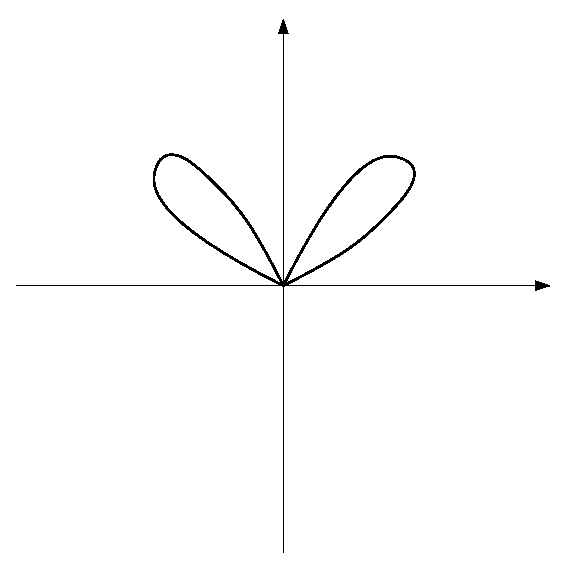
\includegraphics[width=6cm]{img/finiti/curva_regolare.eps}\\
		\begin{equation*}
			r(t)=\begin{cases}
				x=t(1-t^2)^2\\
				y=t^2(1-t^2)
			\end{cases} t\in[-1,1]
		\end{equation*}
	\end{multicols}
	Una curva è {\color{red}regolare a tratti} se è l'unione di curve regolari
	\begin{equation*}
		\gamma r(t)=\begin{cases}
			x=t^3\\
			y=t^2
		\end{cases} t\in[-1,1] \text{ in $x=0$ c'è una cuspide perciò non è regolare $y=\sqrt[3]{x^2}$}
	\end{equation*}
	$r(t)$ può però essere vista come l'unione di che curve regolari
	\begin{equation*}
		\gamma^\prime r (t)=\begin{cases}
			x=t^3\\
			y=t^2
		\end{cases} t\in [-1,0]
	\end{equation*}
	\begin{equation*}
		\gamma^{\prime\prime} r^{\prime\prime}=\begin{cases}
			x=t^3\\
			y=t^2
		\end{cases} t\in [0,1]
	\end{equation*}
	sostegno nel II quadrante
	\begin{equation*}
		\gamma=\gamma^\prime \vee \gamma^{\prime\prime}
	\end{equation*}
\end{defi}
\subsection{Lunghezza di una curva}
\begin{defi}
	Sia la curva $\gamma$ di equazione $\vec{F}(t)$, essa si definisce
	{\color{red}rettificabile} se esiste finito l'estremo superiore della
	poligonale $L(p)$ al variare della decomposizione.
	\begin{equation}
		sup_DL(\Delta)
	\end{equation}
	Suddivido la curva in tanti segmenti che formano la poligonale $L(D)$.
	All'infittirsi la poligonale approssimo sempre seguo la lunghezza della
	curva.\\
	Se la curva $\vec{F}(t)$ è di classe $c^1$ allora essa è
	{\color{red}rettificabile}
	\begin{equation}
		\vec{F}(t)=\begin{cases}
			x=x(t)\\
			y=y(t)\\
			z=z(t)
		\end{cases} t\in [a,b]
	\end{equation}
	e la sua lunghezza vale
	$L=\int_{a}^{b}\sqrt{[x^\prime(t)]^2+[y^\prime(t)]^2 + [z(t)]^2+\dots dt}$
\end{defi}
\subsection{Lunghezza di una curva in forma cartesiana}
Se la curva $\gamma$ nella forma $\begin{cases}
	x=t\\
	y=f(t)
\end{cases} t\in [a,b]$ ha come sostegno il grafico di $y=f(x)$\\
La lunghezza della curva è $L_\gamma=\int_{a}^{b}\sqrt{1+[f^\prime(x)]^2}dx$
\subsection{Lunghezza di una curva polare}
Se le curve è nella forma 
\begin{equation*}
	\begin{cases}
		e=e(\theta)\\
		\theta_1\leq\theta\leq\theta_2
	\end{cases} 
\end{equation*}
La sua lunghezza vale: 
\begin{equation*}
	L_\gamma
	=\int_{\theta_1}^{\theta_2}\sqrt{\varphi^2(\theta)+[\varphi^\prime(\theta)]^2}
	d\theta
\end{equation*}
\section{Ascissa Curvilinea}
È possibile effettuare combiamenti di parametri per descrivere una curva. Fra
tutte le rappresentazioni parametriche di una curva regolare ha particolare
\textbf{importanza} geometrica quella che {\color{red}l'ascissa curvilinea}.
Prendiamo una curva $\gamma$ di $R^2$ e un suo punto $P_0$
\begin{multicols}{2}
	\includegraphics[width=7cm]{img/finiti/ascissa_curvilinea.eps}\\\\\\\\
	Ad ogni punto $P$ della curva associamo un valore $S(P)$ che è uguale
	alla lunguezza dell'arco di curva congiungente $P_0$ e $P$\\
	Così definendo una corrispondenza biurivoca tra i punti della curva e i
	punti di un certo intervallo $[a,b]$, cosiché se $S(p_1)=a$ $S(P_2)=b$ la
	lunqhezza dell'arco congiungente $P_1$ con $P_2$ è $\abs{b-a}$
\end{multicols}
Sia $(\gamma,\vec{r}(t))$ una curva regolare; definiamo \underline{l'ascissa
curvilinea}\footnote{o lunghezza d'arco} come:
\begin{equation*}
	S(t)= \int_{a}^{t}\sqrt{[x^\prime (\uptau)]+[y^\prime(\uptau)]} d\uptau
\end{equation*}
Per il teorema del calcolo integrale
\begin{equation*}
	\begin{matrix}
		S^\prime(t)=\sqrt{[x^\prime(t)]^2+[y^\prime(t)]^2} & S(t) \text{ è
		integrabile}\\
		S^\prime(t)=\frac{ds}{dt} & S:[a,b]\to [0,L]
	\end{matrix}
\end{equation*}
La lunghezza della curva così vale:
\begin{equation}
	L=\int_{a}^{b}\sqrt{[x^\prime(t)]^2+[y^\prime(t)]^2}=\int dS
\end{equation}
\section{Integrale corvilineo}
Prendiamo una funzione f(x,y) definita in un insieme $D$ e una curva $\gamma$
interno a $D$.
\begin{multicols}{2}
	\includegraphics[width=5cm]{img/finiti/integrale_curvilineo.eps}\\
	Calcoliamo la funzione nella curva $\gamma$ e detterminiamo una curva
	$\Gamma$ dello spazio.\\
	L'area delimitata dal cilindro di basi $\gamma$ e $\Gamma$ se $f(x,y)>0$ è
	il valore {\color{red}dell'integrale curvilineo} di $f(x,y)$ esteso a
	$\gamma$.
\end{multicols}
\subsection{Definizione di integrale curvilineo}
Data una curva regolare $(\gamma, \vec{r}(t))$
\begin{equation}
	\begin{cases}
		x=x(t)\\
		y=y(t)\\
		z=z(t)
	\end{cases} t\in [a,b]
\end{equation} 
e una funzione $f(x,y,z)\in \mathds{C}$ -- definita in $D_1$ con la curva
inclusa $D$, si definisce {\color{red}integrale curvilineo} di $f(x,y,z)$
esteso alla curva
\begin{equation*}
	\int_{\gamma} f(x,y,z) ds=
	\int_{a}^{b}f[x(t),y(t),z(t)]*\sqrt{[x^\prime(t)]^2+[y^\prime(t)]^2+[z^\prime(t)]^2}
	dt
\end{equation*}
\subsection{Baricentro di una curva}
Si definisce {\color{red} baricentro di una curva} quel punto di coordinate
$(x_0,y_0)$ per cui
\begin{equation*}
	\begin{matrix}
		x_0=\frac{1}{L_\gamma}\int_\gamma x ds & y_0=\frac{1}{L_\gamma}
		\int_\gamma yds & \text{con $L_\gamma$ lunghezza della curva $\gamma$}
	\end{matrix}
\end{equation*}
\begin{esempio}
	\begin{equation*}
		\gamma=\begin{cases}
			x=\cos^3t\\
			y=\sin^3 t
		\end{cases} t\in \left[0,\frac{\pi}{2}\right]
	\end{equation*}
	\begin{equation*}
		\begin{matrix}
				L_\gamma=\int_{\gamma}ds=\int_{0}^{\frac{\pi}{2}}\sqrt{(-3\cos^2t\sin
			t)^2+(3\sin^2+\cos t)^2} dt\\
			=\int_{0}^{\frac{\pi}{2}}\sqrt{9\cos^4t\sin^2t+9\sin^4t\cos^2t}dt= 
			\int_{0}^{\frac{\pi}{2}}\sqrt{9\cos^2t\sin^2t}*\sqrt{\cos^2t\sin^2t}
			dt = \int_{0}^{\frac{\pi}{2}}3\cos t\sin t dt\\=\left|
			\frac{3\sin^2t}{2}\right|_{0}^{\frac{\pi}{2}}=\frac{3}{2}
		\end{matrix}
	\end{equation*}
	\begin{equation*}
		\begin{matrix}
			x_0=\frac{1}{L_\gamma}\int_\gamma xds=\frac{2}{3}3\cos^4t\sin tdt=
			-\frac{2}{4}\int_{0}^{\frac{\pi}{2}}-4\sin t*\cos^4tdt\\
			y_0=\frac{1}{L_\gamma}\int_\gamma
			yds=\frac{2}{3}\int_{0}^{\frac{\pi}{2}}3\sin^2t+\cos t
			dt=\frac{2}{4}\int_{0}^{\frac{\pi}{2}}4\sin^4t\cos t
			dt=\frac{1}{10} \left|\sin^5t\right|_0^{\frac{\pi}{2}}=\frac{1}{10}
		\end{matrix}
	\end{equation*}
\end{esempio}
\subsection{Superfici e integrali di superficie}
\subsubsection{Superfici}
\begin{defi}
Sia definizsce {\color{red}superfice} in $R^3$ una coppia $(\Sigma, r)$ dove
$\Sigma$ è il sostegno (grafico) $\in R^3$ ed $r$ è la parametrizzazione 
$d\Sigma, r\in\mathds{C}^0_{\dot{A}}.$\\
	$\dot{A}$ insieme aperto connesso di $R^2$ per cali $r(A)=\Sigma$, $r$
	calcolata nei punti di $A$ e da la superficie. $r$ è un'applicazione
	vettoriale
	$r(u,v)=(x(u,v),y(u,v),z(u,v))=x(x,v)\vec{L}+y(u,v)\vec{J}+z(u,v)\vec{k}$
	$(u,v)\in A$ $R^2\to R^3$ ad ogni punto di $A$ del piano, associo un punto
	di $\Sigma$ nello spazio.\\
	Una superficie si dice {\color{red}semplice} $\vec{r}(u,v)$ è 1-1, cioè se
	$x(u,v),y(u,v),z(u,v)$ sono 1-1 (cioè biurivoche, invertite) -- Una
	superficie si dice {\color{red}regolare a tratti} se è firmata dall'unione
	di un numero finito di superfici di classe $C^1$ regolari.\\
	Una superficie è di classe $C^k_A$ se $\vec{r}(u,v)\in C_A^k$ cioè
	$\begin{cases}
		x=x(u,v)\\
		y=y(u,v)\\
		z=z(u,v)
	\end{cases} \in c_A^k$\\
	Una superficie si dice {\color{red}vegolare} se $\vec{r}(u,v)\in C^\prime$
	e la matrice delle derivate parziali prime ha rango 2\\
	Una superficie si dice {\color{red}chiusa} se è limitata e il suo bordo è
	l'insieme ruoto (non ha bordo).
\end{defi}
\begin{teorema}
	Le superfici cartesiane di classe $c^1$ sono regolari:
	\begin{esempio}
		\begin{equation*}
			\begin{matrix}
				\text{Superficie sferica: } &z=\pm\sqrt{R^2+x^2-y^2}&
				x^2+y^2+z^2=R^2 & \text{definita su } D:\{x^2+y^2\leq R^2\}\\
				\text{Superficie corta: } & z=k\sqrt{x^2+y^2}
			\end{matrix}
		\end{equation*}
	\end{esempio}
\end{teorema}
\subsection{Piano tangente e versore normale}
Prendiamo un dominio $A<R^2$ e un suo punto $P(u_0,v_0)$. Prendo due linee in A
passanti per P, sulla superficie $\Sigma$ ho due curve.\\
Sia $\vec{r}(u,v)$ l'equazione della superficie $\Sigma$ e siano
$\vec{r}(u_0,v)$  e $\vec{r}(u,v_0)$ le surve che si chiamano\\ \underline{linee
coordinate superficie}\footnote{(u,v) si chiamano coordinate locali}, i vettori
tangenti alle linee coordinate sono 
\begin{multicols}{2}
	\begin{equation*}
	\begin{matrix}
		\vec{r}_u=(x_u,y_u,z_u)\\
		\vec{r}_v=(x_v,y_v,z_v)
	\end{matrix}
	\end{equation*}
	Se il prodotto vettoriale non è nullo, i vettori sono linearmente ma
	pendenti, quindi il rango di quella matrice è 2. Allora possiamo dire una
	superficie $\sigma$ è regolare se e solo se $\vec{r}_u\wedge \vec{r}_v\neq
	0$, cioè esiste il {\color{red}piano tangente}. $\vec{r}_u\wedge \vec{r}_v$
	e un vettore ortogonale al piano ccontenente $\vec{r}_u$ e $\vec{r}_v$ che
	è il {\color{red}piano tangente} alla superficie.
\end{multicols}
La sua equazione è:\begin{equation*}
	\begin{vmatrix}
		x-x_0 & y-y_0 & z-z_0\\
		x_u & y_u & z_u\\
		x_v & y_v & z_v
	\end{vmatrix} =0\text{ in }P(x_0,y_0,z_0)
\end{equation*}
Per avere il {\color{red}versore normale} si divide il prodotto vettoriale per
la sua lunghezza.
\begin{equation*}
	\vec{n}=\frac{\vec{r}_u \wedge \vec{r}_v}{||\vec{r}_u\wedge \vec{r}_v||}
\end{equation*}
In forma cartesiana
\begin{equation*}
	\begin{matrix}
		\vec{r}(u, v) = \begin{cases}
			x=u\\
			y=v\\
			z=f(u, v)=f(x,y) 
		\end{cases}&r_u=r_x=\begin{cases}
			1 \\
			0\\
			f_x
		\end{cases} & r_v=r_y=\begin{cases}
			0\\
			1\\
			f_y
		\end{cases}
	\end{matrix}
\end{equation*}
Il prodotto vettoriale 
\begin{equation*}
	\vec{r}_x\wedge \vec{r}_y=\begin{vmatrix}
		\vec{i} & \vec{v} &\vec{k}\\
		1 & 0 & f_x\\
		0 & 1 &f_y
	\end{vmatrix}=-f_x\vec{i}-f_y\vec{j}+k=(-f_x;-f_y;1)
\end{equation*}
il versore normale
\begin{equation*}
	\vec{n}=\frac{\vec{r}_x\wedge \vec{r}_y}{||r_x\wedge r_y||}
\end{equation*}
\subsection{Orientazione di una superficie}
Sia $\Sigma$ una superficie regolare $(\vec{r}\in e^\prime, P(M)=2)$, si
scegla il versore normale in modo che vanando con continuità lungo una curva
chiusa $\gamma$ inclusa in $\Sigma_1$ possa ritornare alla posizione inziale in
conseguenza della scelta del versore normale in conseguenza della scelta del
versore normale. Una superficie cartesiana è orientabile.\\
Orientamenti possibili sono: versore normale $\vec{n}$ rivolto verso l'alto o
il verso basso. 
\subsubsection{Area di una superficie}
Sia $\Sigma$ una superficie regolare. Si definisce {\color{red}area della
superficie} $\Sigma$ il numero reale non negativo definito da
\begin{equation*}
	S=\iint_\Sigma d o = \iint_A||\vec{r}_u\wedge
	\vec{r}_vdudv=\iint_A\sqrt{A^2+B^2+C^2}dudv
\end{equation*}
$A,B,C$ componenti del prodotto vettoriale, $d_o$ elemento infinitesimo di
area.\\
Se la superficie $\Sigma$ è in forma cartesiana $z=f(x,y)$ $(x,y)\in D$\\
L'area di $\Sigma$ è
\begin{equation*}
	S=\iint_D \sqrt{1+f_x^2+f_y^2} dxdy
\end{equation*}
Se la superficie $\Sigma$ è data in forma implicità $F(x,y)=0$\\
Con $F_z=0$ per il teorema del Din è localmente esplicitabile in $z=f(x,y)$\\
L'area di $\sigma$ è:
\begin{equation*}
	S=\iint_D\sqrt{1+\left(\frac{F_x}{F_z}\right)^2+\left(\frac{F_y}{F_z}\right)^2}dxdy
\end{equation*}
\subsection{Integrale Superficiale}
Sia $h(x,y,z)$ una funzione definita e continua in un insieme $V \subset R^3$ e
sia $\Sigma$ una superficie inclusa in $V$, che si prosetta in un dominio piano
D. Si definisce {\color{red}integrale superficiale} della funzione $h(x,y,z)$\\
esteso alla superficie $\Sigma$:
\begin{equation*}
	\iint_\Sigma h(x,y,z)do=\iint_A h(x(u, v), y(u, v), z(u, v))||\vec{r}_u\wedge
	\vec{r}_v|| dudv
\end{equation*}
Se la superficie $\Sigma$ è in forma cartesiana
\begin{equation*}
	\iint_\Sigma h(x,y,z)do=\iint_A h(x, y, z(u, v))\sqrt{1+fx^2+f_y^2} dxdy
\end{equation*}
\clearpage
\section{Trasformazione integrali}
\subsection{Formule di Green-Gauss\label{fGreen-Gauss}}
\subsubsection{Prima formula - teorema}
\begin{defi}
	Sia $f(x,y)$ continua in un insieme D, sia $\frac{\partial f}{\partial x}$
	(derivata parziale rispetto a $x$) continua in $D$, sia D normale rispetto all'asse
	$y$ e sia la sua frontiera $F_0$ una curva regolare a tratti\\
	Allora vale la seguente relazione 
	\begin{equation*}
		\iint_{D}\frac{\partial f}{\partial x} dxdy=\int_{FD} f(x,y)dy
	\end{equation*}
	\textbf{FD}: frontiera percorsa nel verso positivo 
	\begin{multicols}{2}
		\paragraph{Ipotesi:}
		\begin{equation*}
			\begin{matrix}
				f(x,y)\in C^o_D\\
				\frac{\partial f}{\partial x}\in C_D^o\\
					\text{D normale rispetto all'asse }y & D: \begin{cases}
						c\leq y\leq d\\
						\alpha (y) \leq x \leq \beta (y)
					\end{cases}\\
					F_D \text{ regolare a tratti}
			\end{matrix}
		\end{equation*}
		\paragraph{Tesi:}
		\begin{equation*}
			\displaystyle\iint_D \frac{\partial f}{\partial x} dxdy=\int_{+FD}
			f(x,y)dy
		\end{equation*}
	\end{multicols}
\end{defi}
\begin{proof}
	Poiché $f(x,y)\in C^o_D$ e $\frac{\partial f}{\partial x}\in C^o_D$, esse
	sono integrabili in D\\
	Il dominio $D_1$ che è normale ripsetto all'asse y, può essere descritto
	come 
	\begin{multicols}{2}
		\includegraphics[width=6cm]{img/finiti/primaLeggeGreenGauss.eps}\\
		\begin{equation*}
			D:\begin{cases}
				c\leq y\leq d\\
				\alpha(y) \leq x \leq \beta (y)
			\end{cases} 
			\begin{matrix}
				\text{ e la sua frontiera è }\\ FD=\gamma_1\cup\gamma_2
			\cup \gamma_3 \cup \gamma_4
			\end{matrix}
		\end{equation*}
	\end{multicols}
	Sviluppiamo I e II membro della tesi
	\begin{description}
		\item[I membro] 
			\begin{equation*}
				\iint_{D} \frac{\partial f}{\partial x} dxdy=\int_{c}^{d}
				dy\int_{\alpha(y)}^{\beta(y)}\frac{\partial f}{\partial x} dx=
				\int_{c}^{d} f[\beta(y),y]-f[\alpha(y),y] dy
			\end{equation*}
			\begin{equation*}
				N.B.\text{ } \int_{\alpha (y)}^{\beta (y)} \frac{\partial
				f}{\partial x} dx=\left| f(x,y) \right|^{x=\beta(y)}_{x=\alpha
				(y)}=f(\beta(y),y)-f(\alpha(y), y)
			\end{equation*}
		\item[II membro]
			$F_D: \gamma_1 \cup \gamma_2 \cup \gamma_3 \cup\gamma_4$
			\begin{equation}
				\int_{+FD}f(x,y)dy=\int_{\gamma_1}f(x,y)dy+\int_{\gamma_2}f(x,y)
				dy+\int_{\gamma_3}f(x,y)dy+\int_{\gamma_4}f(x,y)dy
			\end{equation}
			\begin{multicols}{2}
				\begin{equation*}
					\begin{matrix}
						\begin{matrix}
							\gamma_1: y=c & dy=0
						\end{matrix}\\
						\gamma_2=\begin{cases}
							x=\beta(y)\\
							y\in[c,d]
						\end{cases}
					\end{matrix}
				\end{equation*}
				\begin{equation*}
					\begin{matrix}
						\begin{matrix}
							\gamma_3: y=d & dy=0
						\end{matrix}\\
						\gamma_4=\begin{cases}
							x=\alpha(y)\\
							y\in[d,c]
						\end{cases}
					\end{matrix}
				\end{equation*}
			\end{multicols}
			\begin{equation*}
				\int_{+FD}f(x,y)dy=\int_{\gamma_2}f(x,y)dy+\int_{\gamma_4}f(x,y)
				dy
			\end{equation*}
			\begin{equation*}
				\begin{matrix}
					\int_{\gamma_2}f(x,y)dy=\int_c f[\beta,y]dy &
					\int_{\gamma_4}f(x,y)dy=\int_{d}^{c}f[\alpha(y),y]dy=
					-\int_{c}^{d}f[\alpha(y),y]dy
				\end{matrix}
			\end{equation*}
			\begin{equation*}
				\int_{+FD}f(x,y)dy=\int_{c}^{d}f[\alpha(y),y]dy-
				\int_{c}^{d}f[\alpha(y),y]dy=\int_{c}^{d}f[\alpha(y),y]-
				f[\alpha(y),y]dy
			\end{equation*}
	\end{description}
	Si è così dimostrata la tesi\\
	Per cui con questa {\color{red}formula di Green-Gauss} un integrale doppio
	-- sotto opportune ipotesi -- si può trasformare in un integrale curvilineo
	esteso alla frontiera del dominio di integrazione
	\begin{equation*}
		\iint_D \frac{\partial f}{\partial x}dxdy=\int_{+F_D}f(x,y)dy
	\end{equation*}
\end{proof}
\begin{esempio}
	Calcolare $\iint_D\frac{dxdy}{\sqrt{1-x^2}}$ con $D=\begin{cases}
		xy\leq \frac{1}{4}\\
		x\geq 4\\
		0\leq x\leq \frac{\sqrt{3}}{2}
	\end{cases}$
	\begin{equation*}
		\begin{matrix}
			f(x,y)=\int\frac{1}{\sqrt{1-x^2}}dx=\arcsin x & \to \iint_D
			\frac{dxdy}{\sqrt{1-x^2}}=\int_{+F_D}\arcsin x dy & F_D=
			F_D=\gamma_1\cup \gamma_2 \cup \gamma_3
		\end{matrix}
	\end{equation*}
	\begin{figure}[ht]
		\centering
		\includegraphics[width=6cm]{img/finiti/greenes.eps}
		\caption{Esempio della prima formula di Green-Gauss}
	\end{figure}
	\begin{equation*}
		\begin{matrix}
			\gamma_1: x=\frac{\sqrt{3}}{2} &
			y\in\left[\frac{\sqrt{3}}{6},\frac{1}{2}\right] & \int_{\gamma_1}\arcsin x dy=0
			& \text{ poiché } dy=0 (y=\cos t)\\
			\gamma_2: y=x & x\in \left[\frac{1}{2}, \frac{\sqrt{3}}{2}\right] &
			\text{da percorrere "al contrario"} & dy=d(x)=1dx
		\end{matrix}
	\end{equation*}
\begin{equation*}
	\begin{matrix}
		-\int_{\gamma_2} \arcsin x dy=-\int_{\frac{1}{2}}^{\frac{\sqrt{3}}{2}}
		\arcsin x dx = -\left| x\arcsin x - \int
		\frac{x}{\sqrt{1-x^2}}dx\right|_{\frac{1}{2}}^{\frac{\sqrt{3}}{2}}= 
		-\left| x\arcsin x - \int
		\sqrt{1-x^2}dx\right|_{\frac{1}{2}}^{\frac{\sqrt{3}}{2}}\\
		= -
		\left[\frac{\sqrt{3}}{2}\arcsin\frac{\sqrt{3}}{2}-\sqrt{1-\frac{3}{4}}
		- \frac{1}{2}\arcsin \frac{1}{2}-\sqrt{1-\frac{1}{4}} \right] =
		-\left[\frac{\sqrt{3}}{2}\frac{\pi}{6}+\frac{1}{2}-\frac{1}{2}
		\frac{\pi}{3} - \frac{\sqrt{3}}{2}\right]\\
	\end{matrix}
\end{equation*}
\begin{equation*}
	\begin{matrix}
		\gamma_3: &y=\frac{1}{4x}& x\in \left[\frac{1}{2},
		\frac{\sqrt{3}}{2}\right] & dy=-\frac{1}{4x} & \int_{\gamma_3}\arcsin
		xdy=\int_{\frac{1}{2}}^{\frac{\sqrt{3}}{2}}\arcsin x
		\left(\frac{1}{4x}dx\right)
	\end{matrix}
\end{equation*}
\clearpage
\begin{equation*}
	\begin{matrix}
		\int_{\gamma_3}\arcsin x
		dy=-\int_{\frac{\sqrt{3}}{6}}^{\frac{1}{2}}=y\arcsin \frac{1}{4y}dy=
		y\arcsin \frac{1}{4y}-\int
		y*\frac{1}{\sqrt{1-\frac{1}{16}}y^2}\left(-frac{1}{4y^2}\right)dy\\
		=y\arcsin\left(\frac{1}{4y}\right)-\int-\frac{1}{4y}\frac{1}{\sqrt{\frac{16
		y^2-1}{16y^2}}}dy
	\end{matrix}
\end{equation*}
	Si risolve con la sostituzione $\int\frac{1}{\sqrt{x^2-a^2}}dx$ 
\begin{align*}
	x=\sqrt{x^2-a^2}=a\tan t\\
	\sqrt{y^2-\frac{1}{16}}=\frac{1}{4}\tan t
\end{align*}
\end{esempio}
\subsubsection{Seconda formula di Green-Gauss}
\begin{teorema}
	Sia $f(x,y)$ continua in un insieme D, sia $\frac{\partial f}{\partial y}$
	continua in D, sia D un dominio normale rispetto all'asse x e sia la sua
	frontiera $F_D$ una curva regolarea tratti. Allora vale la seguente
	relazione 
	\begin{equation}
		\iint_D \frac{\partial f}{\partial y} dxdy=-\int_{+FD} f(x,y) dx
	\end{equation}
	\begin{multicols}{2}
		\subsubsection{Ipotesi}
			\begin{equation*}
				\begin{matrix}
					f(x,y)\in C^o_D\\
					\frac{\partial f}{\partial y}\in C^0_D
				\end{matrix}
			\end{equation*}
			$D$ normale rispetto all'asse $x$
			\begin{align*}
			D:\begin{cases}
				a\leq x\leq b\\
				g(x)\leq y\leq h(x)
			\end{cases}
			\end{align*}
			$F_D$ regolare a tratti
		\subsubsection{Tesi}
		\begin{equation*}
			\iint_D \frac{\partial f}{\partial y} dxdy=-\int_{+FD} f(x,y)dx
		\end{equation*}
	\end{multicols}
\end{teorema}
\begin{proof}
	Purché $f(x,y)\in C_D^o$ e $\frac{\partial f}{\partial y}\in C_D^o$, esse
	sono integrali in $D$. Il dominio $D_1$ che è normale rospetto all'esse x
	può essere descritto come
	\begin{multicols}{2}
		\includegraphics[width=6cm]{img/finiti/secondalegge.eps}\\
		\begin{equation*}
			D=\begin{cases}
				a\leq x\leq b\\
				g(x)\leq y\leq h(x)
			\end{cases}\begin{matrix}
				\text{ e la sua frontiera è}\\
				F_D=\gamma_1\wedge \gamma_2 \wedge \gamma_3 \wedge \gamma_4
			\end{matrix}
		\end{equation*}
	\end{multicols}
	Svuluppiamo I e II membro della tesi $\int_{h(x)}^{g(x)}\frac{\partial
	f}{\partial y} dy=|f(x,y)|^{y=h(x)}_{y=g(x)}=f[x,h(x)]-f[x,g(x)]$
	\begin{description}
		\item[I membro]
			\begin{equation*}
				\iint_D \frac{\partial f}{\partial y} dx dy=\int_{a}^{b} dx
				\int_{g(x)}^{h(x)}\frac{\partial f}{\partial y} dy=
				f[x,h(x)]-f[x,g(x)]dx
			\end{equation*}
		\item[II membro]
			\begin{equation*}
				\int_D f(x, y) dx = \int_{\gamma_1} f(x,y)dx+\int_{\gamma_2}
				f(x,y)dx+\int_{\gamma_3} f(x,y)dx+\int_{\gamma_4} f(x,y)dx
			\end{equation*}
			\begin{equation*}
				\begin{matrix}
					\gamma_2: &x=b& y\in[g(b),h(b)]dx=0\\
					\gamma_4: &x=a& y\in[g(a),b(a)]dx=0
				\end{matrix}
			\end{equation*}
			\clearpage
			\begin{equation*}
				\begin{matrix}
					\gamma_1: &y=g(x)&x\in[a,b]&\int_{\gamma_1}f(x,y) dx= 
					\int_{a}^{b}f[x,g(x)]dx\\
					\gamma_3: &y=h(x)& x\in[b, a] & \int_{\gamma_3}f(x,y)dx=-\int_{a}^{b}f[x,h(x)]dx
				\end{matrix}
			\end{equation*}
			per cui
			\begin{equation*}
				\int_{+FD}
				f(x,y)dx=\int_{a}^{b}f[x,g(x)]dx-\int_{a}^{b}f[x,h(x)]dx =
				\int_{a}^{b}f[x,g(x)]-f[x,h(x)]dx
			\end{equation*}
	\end{description}
	combiando di segno si dimostra la tesi\\
	con questa formula di {\color{red}Green-Gaun} un integrale doppio -- sotto
	opportune ipotesi -- si può trasformare in un integrale curvilineo hteso
	alla frontiera del dominio di integrazione.
	\begin{equation*}
		\iint \frac{\partial f}{\partial y}dxdy=-\int_{FD} f(x,y) dx
	\end{equation*}
\end{proof}
\subsection{Teorema della divergenza}
\begin{defi}
	Sia $\vec{F}\equiv (f(x,y),g(x,y))\in C^\prime_D$ funzione vetoriale, si
	definisce {\color{red}divergenza} di $\vec{F}$
	\begin{equation*}
		\begin{matrix}
			div \vec{F}=\frac{\partial f}{\partial x}+\frac{\partial
			f}{\partial y} & \begin{matrix}
				\text{derivata rispetto } \partial x \text{ della prima
				componente più derivata}\\
				\text{ rispetto a } \partial y \text{ della
				seconda componente}
			\end{matrix}
		\end{matrix}
	\end{equation*}
\end{defi}
\subsubsection{Teorema della divergenza \label{tdiv}}
\begin{teorema}
	Sia $\vec{F}\equiv (f(x,y), g(x,y))\in C_0^\prime$ e sia D un dominio
	normale\footnote{rispetto ad entrambi gli assi}, con la sua frontiera $F_D$
	regolare a tratti, vale la sequente relazione:
	\begin{equation*}
		\begin{matrix}
			\iint_D div \vec{F}dxdy=\int_{+FD}\vec{F}*\vec{n}ds & \text{ con }
			\vec{n} \text{ versore normale a } F_D
		\end{matrix}
	\end{equation*}
	\begin{multicols}{2}
		\subsubsection{Ipotesi:}
		\begin{equation*}
			\vec{F}\equiv (f(x,y), g(x,y))\in C_0^\prime
		\end{equation*}
		$D$ normale rispetto ad entrambi gli assi $F_D$ regolare a tratti.
		\subsubsection{Tesi:}
		\begin{equation*}
			\iint_D div \vec{F}dxdy=\int_{+FD}\vec{F}*\vec{n}ds
		\end{equation*}
	\end{multicols}
\end{teorema}
\begin{proof}
	\begin{equation*}
		\begin{matrix}
			\iint div \vec{F} dxdy=\iint_{D} \left(\frac{\partial f}{\partial
			x}\right)dxdy & \text{per definizione divergenza}
		\end{matrix}
	\end{equation*}
	Dalle ipotesi valgono le due formule di \textit{\color{red}Green-Gauss}
	\begin{equation*}
		\begin{matrix}
			\iint \frac{\partial f}{\partial x}dxdy=\int_{+FD}f(x,y)dy &:&
			\iint_D \frac{\partial f}{\partial y}dxdy=-\int_{+FD}g(x,y)dx
		\end{matrix}
	\end{equation*}
	Devo così dimostrare che $f(x,y)dx-g(x,y)dy=\vec{F}*\vec{n}ds$\\
	Ricavo il versore normale $\vec{n}$: $F_D$ regolare a tratti ed è quindi ed
	è quindi esprimibile come unione di curve regolari di espressione
	parametrica
	\begin{equation*}
		\begin{matrix}
			\begin{cases}
				x=x(t)\\
				y=y(t)
			\end{cases} t\in [a,b] & \exists x^\prime(t).y^\prime(t)\text{ perché la
			curva è regolare.}

		\end{matrix}
	\end{equation*}
	Il vettore tangente $\vec{t}=(x^\prime(t),y^\prime(t))$, scambiando le
	componenti e cambiandone una di segno si ottine il vettore normale
	$(y^\prime(t),-x^\prime (t))$; dividendo per la norma
	$\sqrt{[x^\prime(t)]^2+[y^\prime(t)]^2}$ si ha il versore normale $\vec{n}$
	\begin{equation*}
		\vec{n}\equiv
		\left(\frac{y^\prime(t)}{\sqrt{[x^\prime(t)]^2+[y^\prime(t)]^2}}:
		\frac{x^\prime (t)}{\sqrt{[x^\prime(t)]^2+[y^\prime(t)]^2}}\right)
	\end{equation*}
	Svolgo ora il prodotto scalere $\vec{F}*\vec{n}ds$, ricordando che
	$ds=\sqrt{[x^\prime(t)]^2+[y^\prime(t)]^2}$ 
	\begin{align*}
		\vec{F}\equiv (f(x,y), g(x,y))\\
		\vec{F}*\vec{n}ds=\left(\frac{f(x,y)y^\prime(t)}{\sqrt{[x^\prime(t)]^2+[y^\prime(t)]^2}}-\frac{g(x,y)x^\prime(t)}{\sqrt{[x^\prime(t)]^2+[y^\prime(t)]^2}}\right)\sqrt{[x^\prime(t)]^2+[y^\prime(t)]^2}
	\end{align*}
	\begin{equation*}
		\begin{matrix}
			\begin{matrix}
				x^\prime(t)=dx\\
				y^\prime(t)=dy
			\end{matrix}&\vec{F}*\vec{n}ds=f(x,y)dy-g(g,y)dx
		\end{matrix}
	\end{equation*}
	Quindi 
	\begin{eqnarray*}
		\iint_D div \vec{F}dxdy=\int_{+FD}f(x,y)dy-g(x,y)dx & div
		\vec{F}=\frac{\partial f}{\partial x}+ \frac{\partial g}{\partial y}
	\end{eqnarray*}
	Il teorema della divergenza (\ref{tdiv}) vale anche in $R^3$, in forma
	vettoriale
	\begin{eqnarray*}
		\iiint_{V}div \vec{F} dxdydz = \iint_{+\Sigma}\vec{F}*\vec{n}ds &\vec{F}
		=\frac{\partial f}{\partial x}+ \frac{\partial g}{\partial y} + 
		\frac{\partial h}{\partial z}
	\end{eqnarray*}
\end{proof}
\begin{esempio}
	calcolare utilizzando il teorema della divergenza $\iint_D div\vec{F}dxdy$
	con $\vec{F}\equiv (-2x^3y;\frac{1}{2}xy), D=\{x^2+y^2\leq 1\}$
	\begin{equation*}
		div \vec{F}=-\frac{2x^3y}{\partial x}+\frac{-\frac{1}{2}xy}{\partial
		y}= -6x^2y-\frac{1}{2}x
	\end{equation*}
	\begin{equation*}
		\iint_D(-6x^2y-\frac{1}{2}x)dxdy=\int_{+FD}f(x,y)dy+g(x,y)dx=\int_{+FD}
		-2x^2ydy+\frac{1}{2}xydx
	\end{equation*}
	\begin{eqnarray*}
		FD:x^2+y^2=1 & \begin{cases}
			x=\cos t \\
			y=\sin t
		\end{cases} t\in [0,2\pi] & \begin{matrix}
			dx=-\sin t dt\\
			dy=\cos t dt
		\end{matrix}
	\end{eqnarray*}
	\begin{eqnarray*}
		\int_{0}^{2\pi} -2\cos^3 t \sin t\cos t dt + \frac{1}{2}\cos t \sin t
		(-\sin t) dt= +\int_{0}^{2\pi} \left(-2\cos^4t\sin t +
		\frac{1}{2}\sin^2t \cos t\right)\\=\begin{vmatrix}
			-\frac{2}{5} \cos^5 t - \frac{7}{6}\sin^3 t
		\end{vmatrix}^{2\pi}_0 =-\frac{2}{5}-0+\frac{2}{5} -0=0
	\end{eqnarray*}
\end{esempio}
\subsubsection{Applicazioni della formula di Green-Gauss}
Rimandi teorici a partire da (\ref{fGreen-Gauss}) -- Calcolo dell'area di
dominio piani\\
Ricordando le formule di \texttt{Green-Gauss} $\iint_D \frac{\partial
f}{\partial x}dxdy=\int_{+FD} f(x,y)dy:\iint_D \frac{\partial f}{\partial
y}dxdy =-\int_{+FD}f(x,y)dx$ nella formula dell'area $\frac{\partial
f}{\partial x}=1$ o $\frac{\partial f}{\partial y}=1$ per cui $f(x,y)=x$ o
$f(x,y)=y$\\
Si ha così $A=\iint_D dxdy=\int_{+FD}xdy=-\int_{+FD}ydx\to
\int_{+FD}xdy-\int_{+FD}ydx=2\iint_Ddxdy$ si ha:
\begin{equation*}
	\boxed{A=\frac{1}{2}\int_{+FD}xdy-ydx}
\end{equation*}
\clearpage
\begin{esempio}
	Calcolare l'area del dominio delimitato dall'ellisse con semiassi a e b
	\begin{eqnarray*}
		F_D:\begin{matrix}
			x=a\cos t \\
			y=b\sin t
		\end{matrix}& t\in [0,2\pi]&\begin{matrix}
			dx=a\sin t \\
			dy=b\cos t
		\end{matrix}
	\end{eqnarray*}
	\begin{eqnarray*}
		\iint dxdy= \frac{1}{2}\int_{+FD}xdy-ydx=\frac{1}{2}\int_{0}^{2\pi}a
		\cos t (b\cos t)- b\sin t (-a \sin
		t)dt\\=\frac{1}{2}\int_{0}^{2\pi}ab\cos^2t+ab\cos^2 t +
		ab\sin^2t=\frac{1}{2}ab\int_{0}^{2\pi}dt=ab\pi
	\end{eqnarray*}
\end{esempio}
